%
% symmetrien.tex -- Geometrische Beschreibung von Symmetrien, O(n), SO(n),
%                   Spiegelungen
%
% (c) 2020 Prof Dr Andreas Müller, Hochschule Rapperswil
%
\section{Symmetrien
\label{buch:section:symmetrien}}
\rhead{Symmetrien}
Der geometrische Begriff der Symmetrie meint die Eigenschaft eines
geometrischen Objektes, dass es bei einer Bewegung auf sich selbst
abgebildet wird.
Das Wort stammt aus dem altgriechischen, wo es {\em Gleichmass}
bedeutet.
Spiegelsymmetrische Objekte zeichnen sich zum Beispiel dadurch aus,
dass Messungen von Strecken die gleichen Werte ergeben wie die Messungen
der entsprechenden gespiegelten Strecken (siehe auch
Abbildung~\ref{buch:lie:bild:castlehoward}, was die Herkunft des
Begriffs verständlich macht.
\begin{figure}
\centering
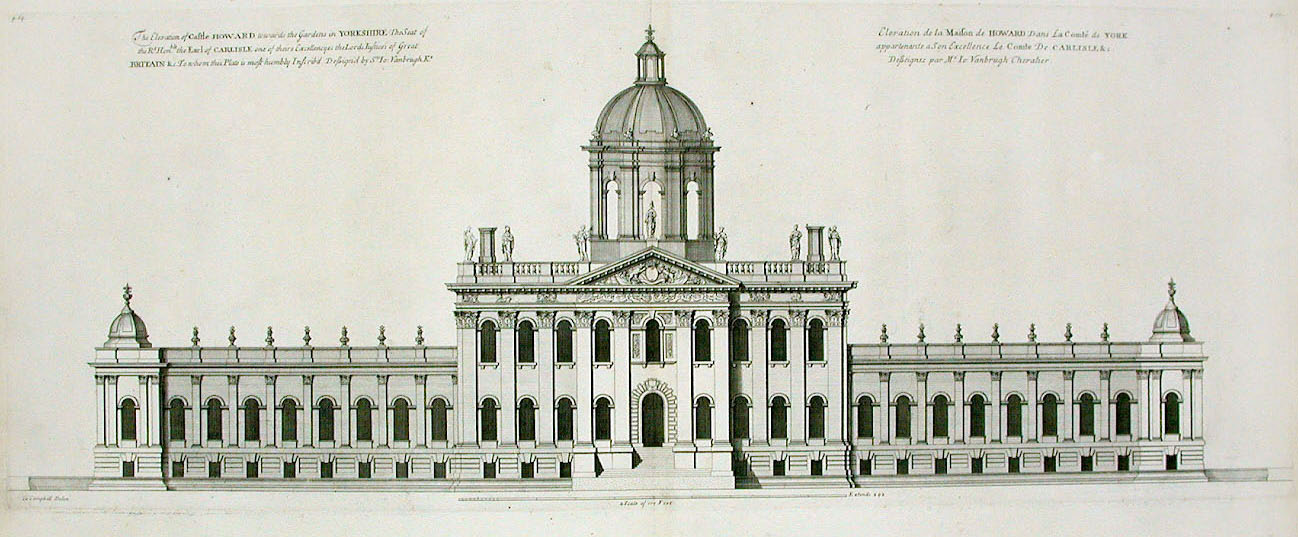
\includegraphics[width=\textwidth]{chapters/60-gruppen/images/castle.jpeg}
\caption{Das Castle Howard in Yorkshire war in dieser ausgeprägt symmetrischen
Form geplant, wurde dann aber in modifizeirter Form gebaut.
Messungen zwischen Punkten in der rechten Hälfte des Bildes
ergeben die gleichen Werte wie Messungen entsprechenden Strecken
in der linken Hälfte, was den Begriff Symmetrie rechtfertigt.
\label{buch:lie:bild:castlehoward}}
\end{figure}
In der Physik wird dem Begriff der Symmetrie daher auch eine erweiterte
Bedeutung gegeben.
Jede Transformation eines Systems, welche bestimmte Grössen nicht
verändert, wird als Symmetrie bezeichnet.
Die Gesetze der Physik sind typischerweise unabhängig davon, wo man den
den Nullpunkt der Zeit oder das räumlichen Koordinatensystems ansetzt,
eine Transformation des Zeitnullpunktes oder des Ursprungs des
Koordinatensystems ändert daher die Bewegungsgleichungen nicht, sie ist
eine Symmetrie des Systems.

Umgekehrt kann man fragen, welche Symmetrien ein System hat.
Da sich Symmetrien zusammensetzen und umkehren lassen, kann man in davon
ausgehen, dass die Symmetrietransformationen eine Gruppe bilden.
Besonders interessant ist dies im Falle von Transformationen, die
durch Matrizen beschrieben weren.
Eine unter der Symmetrie erhaltene Eigenschaft definiert so eine
Untergruppe der Gruppe $\operatorname{GL}_n(\mathbb{R})$ der
invertierbaren Matrizen.
Die erhaltenen Eigenschaften definieren eine Menge von Gleichungen,
denen die Elemente der Untergruppe genügen müssen.
Als Lösungsmenge einer Gleichung erhält die Untergruppe damit eine
zusätzliche geometrische Struktur, man nennt sie eine differenzierbare
Mannigfaltigkeit.
Dieser Begriff wird im Abschnitt~\ref{buch:subsection:mannigfaltigkeit}
eingeführt.
Es wird sich zum Beispiel zeigen, dass die Menge der Drehungen der
Ebene mit den Punkten eines Kreises parametrisieren lassen,
die Lösungen der Gleichung $x^2+y^2=1$ sind.

Eine Lie-Gruppe ist eine Gruppe, die gleichzeitig eine differenzierbare
Mannigfaltigkeit ist.
Die Existenz von geometrischen Konzepten wie Tangentialvektoren
ermöglicht zusätzliche Werkzeuge, mit denen diese Gruppe untersucht
und verstanden werden können.
Ziel dieses Abschnitts ist, die Grundlagen für diese Untersuchung zu
schaffen, die dann im Abschnitt~\ref{buch:section:lie-algebren}
durchgeführt werden soll.

\subsection{Algebraische Symmetrien
\label{buch:subsection:algebraische-symmetrien}}
Mit Matrizen lassen sich Symmetrien in einem geometrischen Problem
oder in einem physikalischen System beschreiben.
Man denkt dabei gerne zuerst an geometrische Symmetrien wie die
Symmetrie unter Punktspiegelung oder die Spiegelung an der $x_1$-$x_2$-Ebene,
wie sie zum Beispiel durch die Abbildungen
\[
\mathbb{R}^3\to\mathbb{R}^3 : x\mapsto -x
\qquad\text{oder}\qquad
\mathbb{R}^3\to\mathbb{R}^3 :
\begin{pmatrix}x_1\\x_2\\x_3\end{pmatrix}
\mapsto
\begin{pmatrix}-x_1\\x_2\\x_3\end{pmatrix}
\]
dargestellt werden.
Beide haben zunächst die Eigenschaft, dass Längen und Winkel und damit
das Skalarprodukt erhalten sind.
Diese Eigenschaft allein erlaubt aber noch nicht, die beiden Transformationen
zu unterscheiden.
Die Punktspiegelung zeichnet sich dadurch aus, das alle Geraden und alle
Ebenen durch den Ursprung auf sich selbst abgebildet werden.
Dies funktioniert für die Ebenenspiegelung nicht, dort bleibt nur die
Spiegelungsebene (die $x_1$-$x_2$-Ebene im vorliegenden Fall) und
ihre Normale erhalten.
Die folgenden Beispiele sollen zeigen, wie solche Symmetriedefinitionen
auf algebraische Bedingungen an die Matrixelemente führen.

Zu jeder Abbildung $f\colon\mathbb{R}^n\to\mathbb{R}^n$, unter der 
ein geometrisches Objekt in $\mathbb{R}^n$ symmetrisch ist, können wir
sofort weitere Abbildungen angeben, die ebenfalls Symmetrien sind.
Zum Beispiel sind die iterierten Abbildungen $f\circ f$, $f\circ f\circ f$
u.~s.~w., die wir auch $f^n$ mit $n\in\mathbb{N}$ schreiben werden,
ebenfalls Symmetrien.
Wenn die Symmetrie auch umkehrbar ist, dann gilt dies sogar für alle
$n\in\mathbb{Z}$.
Wir erhalten so eine Abbildung
$\varphi\colon \mathbb{Z}\to \operatorname{GL}_n(\mathbb{R}):n\mapsto f^n$
mit den Eigenschaften $\varphi(0)=f^0 = I$ und
$\varphi(n+m)=f^{n+m}=f^n\circ f^m = \varphi(n)\circ\varphi(m)$.
$\varphi$ ist ein Homomorphismus der Gruppe $\mathbb{Z}$ in die Gruppe
$\operatorname{GL}_n(\mathbb{R})$.
Wir nennen dies eine {\em diskrete Symmetrie}.

\subsection{Kontinuierliche Symmetrien
\label{buch:subsection:kontinuierliche-symmetrien}}
Von besonderem Interesse sind kontinuierliche Symmetrien.
Dies sind Abbildungen eines Systems, die von einem Parameter
abhängen.
Zum Beispiel können wir Drehungen der Ebene $\mathbb{R}^2$ um den
Winkel $\alpha$ durch Matrizen 
\[
D_{\alpha}
=
\begin{pmatrix}
\cos\alpha&-\sin\alpha\\
\sin\alpha& \cos\alpha
\end{pmatrix}
\]
beschrieben werden.
Ein Kreis um den Nullpunkt bleibt unter jeder dieser Drehungen invariant.
Im Gegensatz dazu sind alle $3n$-Ecke mit Schwerpunkt $0$ nur invariant
unter der einen Drehung $D_{\frac{2\pi}3}$ invariant.
Die kleinste Menge, die einen vorgegebenen Punkt enthält und unter
allen Drehungen $D_\alpha$ invariant ist, ist immer ein Kreis um
den Nullpunkt.

\begin{definition}
Ein Homomorphismus $\varphi\colon\mathbb{R}\to\operatorname{GL}_n(\mathbb{R})$
von der additiven Gruppe $\mathbb{R}$ in die allgemeine lineare Gruppe
heisst eine {\em Einparameter-Untergruppe} von
$\operatorname{GL}_n(\mathbb{R})$.
\end{definition}

Die Abbildung 
\[
\varphi
\colon
\mathbb{R}\to\operatorname{GL}_n(\mathbb{R})
:
\alpha \mapsto
D_{\alpha}
=
\begin{pmatrix}
\cos\alpha&-\sin\alpha\\
\sin\alpha& \cos\alpha
\end{pmatrix}
\]
ist also eine Einparameter-Untergruppe von $\operatorname{GL}_2(\mathbb{R})$.

\subsubsection{Der harmonische Oszillator}
\begin{figure}
\centering
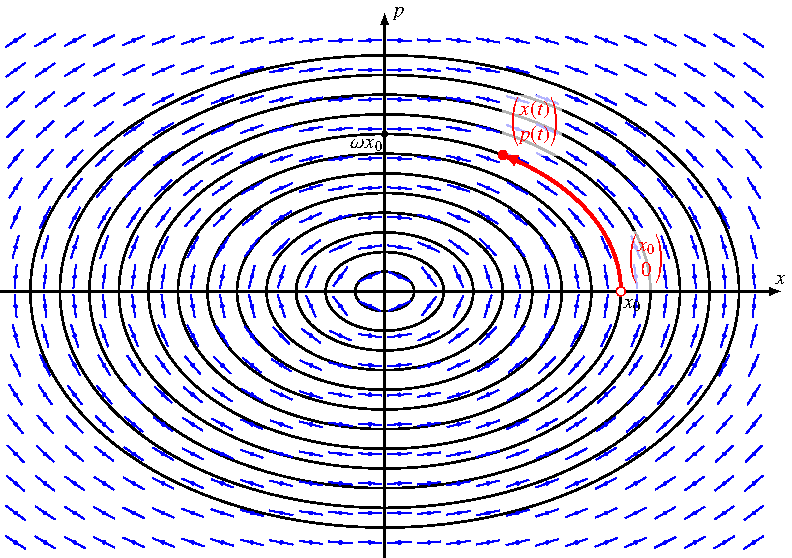
\includegraphics{chapters/60-gruppen/images/phasenraum.pdf}
\caption{Die Lösungen der
Differentialgleichung~\eqref{chapter:gruppen:eqn:phasenraumdgl}
im Phasenraum sind Ellipsen mit Halbachsenverhältnis $\omega^{-1}$.
\label{chapter:gruppen:fig:phasenraum}}
\end{figure}
Eine Masse $m$ verbunden mit einer Feder mit der Federkonstanten $K$
schwingt um die Ruhelage $x=0$ entsprechend der Differentialgleichung
\[
m\frac{d^2}{dt^2} x(t) =  -Kx(t).
\]
Die Kreisfrequenz der Schwingung ist
\[
\omega = \sqrt{\frac{K}{m}}.
\]
Das System kann als zweidimensionales System im Phasenraum mit den 
Koordinaten $x_1=x$ und $x_2=p=m\dot{x}$ beschrieben werden.
Die zweidimensionale Differentialgleichung ist
\begin{equation}
\left.
\begin{aligned}
\dot{x}(t) &= \frac{1}{m}p(t)\\
\dot{p}(t) &= -Kx(t) 
\end{aligned}
\quad
\right\}
\qquad\Rightarrow\qquad
\frac{d}{dt}
\begin{pmatrix}x(t)\\p(t)\end{pmatrix}
=
\begin{pmatrix}
0&\frac{1}{m}\\
-K&0
\end{pmatrix}
\begin{pmatrix}x(t)\\p(t)\end{pmatrix}.
\label{chapter:gruppen:eqn:phasenraumdgl}
\end{equation}
Die Lösung der Differentialgleichung für die Anfangsbedingung $x(0)=1$ und
$p(0)=0$ ist
\[
x(t)
=
\cos \omega t
\qquad\Rightarrow\qquad
p(t)
=
-\omega \sin\omega t,
\]
die Lösung zur Anfangsbedingung $x(0)=0$ und $p(0)=1$ ist
\[
x(t) = \frac{1}{\omega} \sin\omega t,
\qquad
p(t) = \cos \omega t.
\]
In Matrixform kann man die allgemeine Lösung zur Anfangsbedingun $x(0)=x_0$
und $p(0)=p_0$
\begin{equation}
\begin{pmatrix}
x(t)\\
p(t)
\end{pmatrix}
=
\underbrace{
\begin{pmatrix}
 \cos \omega t & \frac{1}{\omega} \sin\omega t \\
-\omega \sin\omega t & \cos\omega t
\end{pmatrix}
}_{\displaystyle =\Phi_t}
\begin{pmatrix}x_0\\p_0\end{pmatrix}
\label{buch:gruppen:eqn:phi}
\end{equation}
schreiben.
Die Matrizen $\Phi_t$ bilden eine Einparameter-Untergruppe von
$\operatorname{GL}_n(\mathbb{R})$, da
\begin{align*}
\Phi_s\Phi_t
&=
\begin{pmatrix}
 \cos\omega s & \frac{1}{\omega} \sin\omega s \\
-\omega \sin\omega s & \cos\omega s
\end{pmatrix}
\begin{pmatrix}
 \cos\omega t & \frac{1}{\omega} \sin\omega t \\
-\omega \sin\omega t & \cos\omega t
\end{pmatrix}
\\
&=
\begin{pmatrix}
\cos\omega s \cos\omega t - \sin\omega s \sin\omega t 
& \frac{1}{\omega} ( \cos\omega s \sin\omega t + \sin\omega s \cos \omega t)
\\
-\omega (\sin\omega s \cos\omega t + \cos\omega s \sin\omega t )
& \cos\omega s \cos\omega t -\sin\omega s \sin\omega t 
\end{pmatrix}
\\
&=
\begin{pmatrix}
 \cos\omega(s+t) & \frac{1}{\omega}\sin\omega(s+t) \\
-\omega \sin\omega(s+t) & \cos\omega(s+t)
\end{pmatrix}
=
\Phi_{s+t}
\end{align*}
gilt.
Die Lösungen der 
Differentialgleichung~\eqref{chapter:gruppen:eqn:phasenraumdgl}
sind in Abbildung~\ref{chapter:gruppen:fig:phasenraum}
Die Matrizen $\Phi_t$ beschreiben eine kontinuierliche Symmetrie
des Differentialgleichungssystems, welches den harmonischen Oszillator
beschreibt.

\subsubsection{Fluss einer Differentialgleichung}
Die Abbildungen $\Phi_t$ von \eqref{buch:gruppen:eqn:phi} sind jeweils
Matrizen in $\operatorname{GL}_n(\mathbb{R})$.
Der Grund dafür ist, dass die
Differentialgleichung~\eqref{chapter:gruppen:eqn:phasenraumdgl}
linear ist.
Dies hat zur Folge, dass für zwei Anfangsbedingungen $x_1,x_2\in\mathbb{R}^2$
die Lösung für Linearkombinationen $\lambda x_1+\mu x_2$ durch
Linearkombination der Lösungen erhalten werden kann, also
aus der Formel
\[
\Phi_t (\lambda x_1 + \mu x_2) = \lambda \Phi_t x_1 + \mu \Phi_t x_2.
\]
Dies zeigt, dass $\Phi_t$ für jedes $t$ eine lineare Abbildung sein muss.

Für eine beliebige Differentialgleichung kann man immer noch eine Abbildung
$\Phi$ konstruieren, die aber nicht mehr linear ist.
Sei dazu die Differentialgleichung erster Ordnung
\begin{equation}
\frac{dx}{dt}
=
f(t,x)
\qquad\text{mit}\qquad
f\colon \mathbb{R}\times\mathbb{R}^n \to \mathbb{R}^n
\label{buch:gruppen:eqn:dgl}
\end{equation}
gegeben.
Für jeden Anfangswert $x_0\in\mathbb{R}^n$ kann man mindestens für eine
gewisse Zeit $t <\varepsilon$ eine Lösung $x(t,x_0)$ finden mit $x(t,x_0)=x_0$.
Aus der Theorie der gewöhnlichen Differentialgleichungen ist auch
bekannt, dass $x(t,x_0)$ mindestens in der Nähe von $x_0$ differenzierbar von
$x_0$ abhängt.
Dies erlaubt eine Abbildung
\[
\Phi\colon \mathbb{R}\times \mathbb{R}^n \to \mathbb{R}^n
:
(t,x_0) \mapsto \Phi_t(x_0) = x(t,x_0)
\]
zu definieren, die sowohl von $t$ als auch von $x_0$ differenzierbar
abhängt.
Aus der Definition folgt unmittelbar, dass $\Phi_0(x_0)=x_0$ ist, dass
also $\Phi_0$ die identische Abbildung von $\mathbb{R}^n$ ist.

Aus der Definition lässt sich auch ableiten, dass
$\Phi_{s+t}=\Phi_s\circ\Phi_t$ gilt.
$\Phi_t(x_0)=x(t,x_0)$ ist der Endpunkt der Bahn, die bei $x_0$ beginnt
und sich während der Zeit $t$ entwickelt.
$\Phi_s(x(t,x_0))$ ist dann der Endpunkt der Bahn, die bei $x(t,x_0)$ 
beginnt und sich während der Zeit $s$ entwickelt.
Somit ist $\Phi_s\circ \Phi_t(x_0)$ der Endpunkt der Bahn, die bei
$x_0$ beginnt und sich über die Zeit $s+t$ entwickelt.
In Formeln bedeutet dies
\[
\Phi_{s+t} = \Phi_s\circ \Phi_t.
\]
Die Abbildung $t\mapsto \Phi_t$ ist also wieder ein Homomorphismus
von der additiven Gruppe $\mathbb{R}$ in eine Gruppe von differenzierbaren
Abbildungen $\mathbb{R}^n\to\mathbb{R}^n$.

\begin{definition}
Die Abbildung
\[
\Phi\colon \mathbb{R}\times\mathbb{R}^n\to\mathbb{R}^n
:
(t,x_0) \mapsto \Phi_t(x_0) = x(t,x_0)
\]
heisst der {\em Fluss} der Differentialgleichung
\eqref{buch:gruppen:eqn:dgl},
wenn für jedes $x_0\in\mathbb{R}^n$ die Kurve $t\mapsto \Phi_t(x_0)$
eine Lösung der Differentialgleichung ist mit Anfangsbedingung $x_0$.
\end{definition}

Die Abbildung $\Phi_t$ von \eqref{buch:gruppen:eqn:phi} ist also
der Fluss der Differentialgleichung des harmonischen Oszillators.

\subsection{Mannigfaltigkeiten
\label{buch:subsection:mannigfaltigkeit}}
Eine Differentialgleichung der Form~\eqref{buch:gruppen:eqn:dgl}
stellt einen Zusammenhang her zwischen einem Punkt $x$ und der
Tangentialrichtung einer Bahnkurve $f(t,x)$.
Die Ableitung liefert die lineare Näherung der Bahkurve
\[
x(t_0+h) = x(t_0) + h f(t_0,x_0) + o(h)
\]
für $h$ in einer kleinen Umgebung von $0$.
Das funktioniert auch, weil $f(t_0,x_0)$ selbst ein Vektor von
$\mathbb{R}^n$ ist, in dem die Bahnkurve verläuft.

Diese Idee funktioniert nicht mehr zum Beispiel für eine
Differentialgleichung auf einer Kugeloberfläche, weil alle Punkte
$x(t_0)+hf(t_0,x_0)$ für alle $h\ne 0$ nicht mehr auf der Kugeloberfläche
liegen.
Physikalisch äussert sich das ein einer zusätzlichen Kraft, die nötig
ist, die Bahn auf der Kugeloberfläche zu halten.
Diese Kraft stellt zum Beispiel sicher, dass die Vektoren $f(t,x)$ für
Punkte $x$ auf der Kugeloberfläche immer tangential an die Kugel sind.
Trotzdem ist der Tangentialvektor oder der Geschwindigkeitsvektor 
nicht mehr ein Objekt, welches als Teil der Kugeloberfläche definiert
werden kann, er kann nur definiert werden, wenn man sich die Kugel als
in einen höherdimensionalen Raum eingebettet vorstellen kann.

Um die Idee der Differentialgleichung auf einer beliebigen Fläche
konsistent zu machen ist daher notwendig, die Idee einer Tagentialrichtung
auf eine Art zu definieren, die nicht von der Einbettung der Fläche
in den $n$-dimensionalen Raum abhängig ist.
Das in diesem Abschnitt entwickelte Konzept der {\em Mannigfaltigkeit}
löst dieses Problem.

\subsubsection{Karten}
Die Navigation auf der Erdoberfläche verwendet das Koordinatensystem
der geographischen Länge und Breite.
Dieses Koordinatensystem funktioniert gut, solange man sich nicht an
den geographischen Polen befindet, denn deren Koordinaten sind
nicht mehr eindeutig.
Alle Punkte mit geographischer Breite $90^\circ$ und beliebiger 
geographischer Länge beschreiben den Nordpol.
Auch die Ableitung funktioniert dort nicht mehr.
Bewegt man sich mit konstanter Geschwindigkeit über den Nordpol,
springt die Ableitung der geographischen Breite von einem positiven
Wert auf einen negativen Wert, sie kann also nicht differenzierbar sein.
Diese Einschränkungen sind in der Praxis nur ein geringes Problem dar,
da die meisten Reisen nicht über die Pole erfolgen.

Der Polarforscher, der in unmittelbarer Umgebung des Poles arbeitet,
kann das Problem lösen, indem er eine lokale Karte für das Gebiet
um den Pol erstellt.
Dafür kann er beliebige Koordinaten verwenden, zum Beispiel auch
ein kartesisches Koordinatensystem, er muss nur eine Methode haben,
wie er seine Koordinaten wieder auf geographische Länge und Breite
umrechnen will.
Und wenn er über Geschwindigkeiten kommunizieren will, dann muss
er auch Ableitungen von Kurven in seinem kartesischen Koordinatensystem
umrechnen können auf die Kugelkoordinaten.
Dazu muss seine Umrechnungsformel von kartesischen Koordinaten
auf Kugelkoordinaten differenzierbar sein.

Diese Idee wird durch das Konzept der Mannigfaltigkeit verallgemeinert.
Eine $n$-dimensionale {\em Mannigfaltigkeit} ist eine Menge $M$ von Punkten,
die lokal, also in der Umgebung eines Punktes, mit möglicherweise mehreren
verschiedenen Koordinatensystemen versehen werden kann.
Ein Koordinatensystem ist eine umkehrbare Abbildung einer offenen Teilmenge
$U\subset M$ in den Raum $\mathbb{R}^n$.
Die Komponenten dieser Abbildung heissen die {\em Koordinaten}.

\begin{figure}
\centering
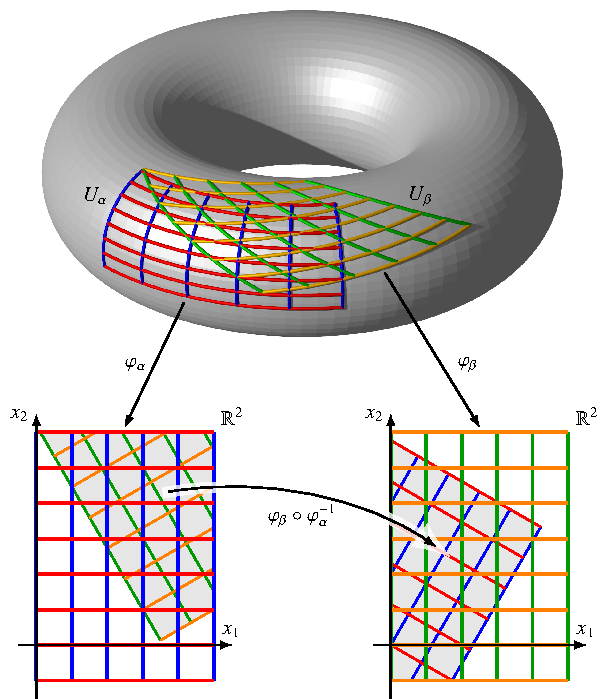
\includegraphics{chapters/60-gruppen/images/karten.pdf}
\caption{Karten
$\varphi_\alpha\colon U_\alpha\to \mathbb{R}^2$
und
$\varphi_\beta\colon U_\beta\to \mathbb{R}^2$
auf einem Torus.
Auf dem Überschneidungsgebiet $\varphi_\alpha^{-1}(U_\alpha\cap U_\beta)$
ist der Kartenwechsel $\varphi_\beta\circ\varphi_\alpha^{-1}$ wohldefiniert
und muss differnzierbar sein, wenn eine differenzierbare Mannigfaltigkeit
entstehen soll.
\label{buch:gruppen:fig:karten}}
\end{figure}

\begin{definition}
Eine Karte auf $M$ ist eine umkehrbare Abbildung
$\varphi\colon U\to \mathbb{R}^n$ (siehe auch
Abbildung~\ref{buch:gruppen:fig:karten}).
Ein differenzierbarer Atlas ist eine Familie von Karten $\varphi_\alpha$
derart, dass die Definitionsgebiete $U_\alpha$ die ganze Menge $M$
überdecken, und dass die Kartenwechsel Abbildungen
\[
\varphi_{\beta\alpha}=\varphi_\beta\circ\varphi_\alpha^{-1}
\colon
\varphi_\alpha(U_\alpha\cap U_\beta)
\to
\varphi_\beta(U_\alpha\cap U_\beta)
\]
als Abbildung von offenen Teilmengen von $\mathbb{R}^n$ differenzierbar
ist.
Eine {$n$-dimensionale differenzierbare Mannigfaltigkeit} ist eine
Menge $M$ mit einem differenzierbaren Atlas.
\end{definition}

Karten und Atlanten regeln also nur, wie sich verschiedene lokale
Koordinatensysteme ineinander umrechnen lassen.

\begin{beispiel}
$M=\mathbb{R}^n$ ist eine differenzierbare Mannigfaltigkeit denn 
die identische Abbildung $M\to \mathbb{R}^n$ ist eine Karte und ein
Atlas von $M$.
\end{beispiel}

\begin{beispiel}
\begin{figure}
\centering
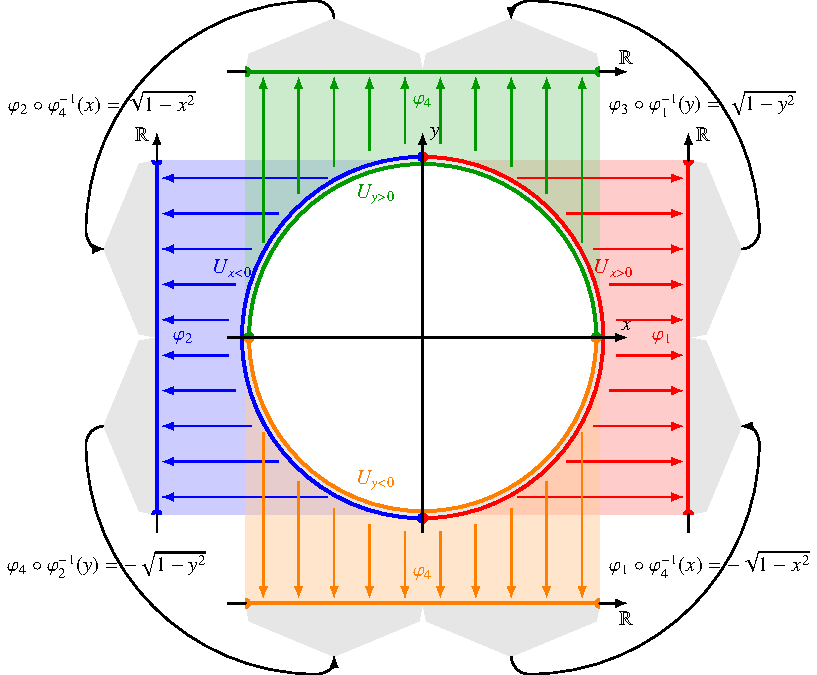
\includegraphics{chapters/60-gruppen/images/kartenkreis.pdf}
\caption{Karten für die Kreislinie $S^1\subset\mathbb{R}^2$.
\label{buch:gruppen:fig:kartenkreis}}
\end{figure}
Die Kreislinie in in der Ebene ist eine $1$-dimensionale Mannigfaltigkeit.
Natürlich kann sie nicht mit einer einzigen Karte beschrieben werden,
da es keine umkehrbaren Abbildungen zwischen $\mathbb{R}$ und der Kreislinie
gibt.
Die Projektionen auf die einzelnen Koordinaten liefern die folgenden
vier Karten:
\begin{align*}
\varphi_1&\colon U_{x>0}\{(x,y)\;|\;x^2+y^2=1\wedge x>0\} \to\mathbb{R}
:
(x,y) \mapsto y
\\
\varphi_2&\colon U_{x<0}\{(x,y)\;|\;x^2+y^2=1\wedge x<0\} \to\mathbb{R}
:
(x,y) \mapsto y
\\
\varphi_3&\colon U_{y>0}\{(x,y)\;|\;x^2+y^2=1\wedge y>0\} \to\mathbb{R}
:
(x,y) \mapsto x
\\
\varphi_4&\colon U_{y<0}\{(x,y)\;|\;x^2+y^2=1\wedge y<0\} \to\mathbb{R}
:
(x,y) \mapsto x
\end{align*}
Die Werte der Kartenabbildungen sind genau die $x$- und $y$-Koordinaten
auf der in den Raum $\mathbb{R}^2$ eingebetteten Kreislinie.

Für $\varphi_1$ und $\varphi_2$ sind die Definitionsgebiete disjunkt,
hier gibt es also keine Notwendigkeit, Koordinatenumrechnungen vornehmen
zu können.
Dasselbe gilt für $\varphi_3$ und $\varphi_4$.

Die nichtleeren Schnittmengen der verschiedenen Kartengebiete beschreiben
jeweils die Punkte der Kreislinie in einem Quadranten.
Die Umrechnung zwischen den Koordinaten und ihre Ableitung
ist je nach Quadrant durch
\begin{align*}
&\text{1.~Quadrant}&
\varphi_{31}
&=
\varphi_3\circ\varphi_1^{-1}\colon y\mapsto\phantom{-}\sqrt{1-y^2\mathstrut}
&
D\varphi_{31}
&=
-\frac{y}{\sqrt{1-y^2\mathstrut}}
\\
&\text{2.~Quadrant}&
\varphi_{24}
&=
\varphi_3\circ\varphi_1^{-1}\colon x\mapsto\phantom{-}\sqrt{1-x^2\mathstrut}
&
D\varphi_{24}
&=
-\frac{x}{\sqrt{1-x^2\mathstrut}}
\\
&\text{3.~Quadrant}&
\varphi_{42}
&=
\varphi_3\circ\varphi_1^{-1}\colon y\mapsto-\sqrt{1-y^2\mathstrut}
&
D\varphi_{42}
&=
\phantom{-}\frac{y}{\sqrt{1-y^2\mathstrut}}
\\
&\text{4.~Quadrant}&
\varphi_{14}
&=
\varphi_3\circ\varphi_1^{-1}\colon x\mapsto-\sqrt{1-x^2\mathstrut}
&
D\varphi_{14}
&=
\phantom{-}\frac{x}{\sqrt{1-x^2\mathstrut}}
\end{align*}
gegeben.
Diese Abbildungen sind im offenen Intervall $(-1,1)$ differenzierbar,
Schwierigkeiten mit der Ableitungen ergeben sich nur an den Stellen
$x=\pm1$ und $y=\pm 1$, die in einem Überschneidungsgebiet von Karten
nicht vorkommen können.
Somit bilden die vier Karten einen differenzierbaren Atlas für
die Kreislinie (Abbildung~\ref{buch:gruppen:fig:kartenkreis}).
\end{beispiel}

\begin{beispiel}
Ganz analog zum vorangegangenen Beispiel über die Kreisline lässt sich
für eine $n$-di\-men\-sio\-nale Sphäre
\[
S^n = \{ (x_1,\dots,x_{n+1})\;|\; x_0^2+\dots+x_n^2=1\}
\]
immer ein Atlas aus $2^{n+1}$ Karten mit den Koordinatenabbildungen
\[
\varphi_{i,\pm}
\colon
U_{i,\pm}
=
\{p\in S^n\;|\; \pm x_i >0\}
\to
\mathbb{R}^n
:
p\mapsto (x_1,\dots,\hat{x}_i,\dots,x_{n+1})
\]
konstruieren, der $S^n$ zu einer $n$-dimensionalen Mannigfaltigkeit macht.
\end{beispiel}

\subsubsection{Tangentialraum}
Mit Hilfe einer Karte $\varphi_\alpha\colon U_\alpha\to\mathbb{R}^n$
kann das Geschehen in einer Mannigfaltigkeit in den vertrauten 
$n$-dimensionalen Raum $\mathbb{B}^n$ transportiert werden. 
Eine Kurve $\gamma\colon \mathbb{R}\to M$, die so parametrisiert sein
soll, dass $\gamma(t)\in U_\alpha$ für $t$ in einer Umgebung $I$ von $0$ ist,
wird von der Karte in eine Kurve
$\gamma_\alpha=\varphi_\alpha\circ\gamma\colon I\to \mathbb{R}^n$ 
abgebildet,
deren Tangentialvektor wieder ein Vektor in $\mathbb{R}^n$ ist.

Eine zweite Karte $\varphi_\beta$ führt auf eine andere Kurve
mit der Parametrisierung
$\gamma_\beta=\varphi_\beta\circ\gamma\colon I \to \mathbb{R}^n$ 
und einem anderen Tangentialvektor.
Die beiden Tangentialvektoren können aber mit der Ableitung der
Koordinatenwechsel-Abbildung
$\varphi_{\beta\alpha}=\varphi_\beta\circ\varphi_\alpha^{-1}\colon
\varphi_\alpha(U_\alpha\cap U_\beta)\to \mathbb{R}^n$
ineinander umgerechnet werden.
Aus
\[
\gamma_\beta
=
\varphi_\beta\circ \gamma
=
(
\varphi_\beta
\circ
\varphi_\alpha^{-1}
)
\circ
\varphi_\alpha\circ\gamma
=
\varphi_{\beta\alpha}
\circ
\varphi_\alpha\circ\gamma
=
\varphi_{\beta\alpha}\circ\gamma_\alpha
\]
folgt durch Ableitung nach dem Kurvenparameter $t$, dass
\[
\frac{d}{dt}\gamma_\beta(t)
=
D\varphi_{\beta\alpha}
\cdot
\frac{d}{dt}\gamma_\alpha(t).
\]
Die Ableitung $D\varphi_{\beta\alpha}$ von $\varphi_{\beta\alpha}$ 
an der Stelle $\gamma_\alpha(t)$ berechnet also aus dem Tangentialvektor
einer Kurve in der Karte $\varphi_\alpha$ den Tangentialvektor der
Kurve in der Karte $\varphi_\beta$.

Die Forderung nach Differenzierbarkeit der Kartenwechselabbildungen
$\varphi_{\beta\alpha}$ stellt also nur sicher, dass die Beschreibung
eines Systemes mit Differentialgleichungen in verschiedenen
Koordinatensystemen auf die gleichen Lösungskurven in der
Mannigfaltigkeit führt.
Insbesondere ist die Verwendung von Karten ist also nur ein Werkzeug,
mit dem die Unmöglichkeit einer globalen Besschreibung einer
Mannigfaltigkeit $M$ mit einem einzigen globalen Koordinatensystem
ohne Singularitäten umgangen werden kann.

\begin{beispiel}
Das Beispiel des Kreises in Abbildung~\ref{buch:gruppen:fig:kartenkreis}
zeigt, dass die Tangentialvektoren je nach Karte sehr verschieden
aussehen können.
Der Tangentialvektor der Kurve $\gamma(t) = (x(t), y(t))$ im Punkt
$\gamma(t)$ ist $\dot{y}(t)$ in den Karten $\varphi_1$ und $\varphi_2$ 
und $\dot{x}(t)$ in den Karten $\varphi_3$ und $\varphi_4$.

Die spezielle Kurve $\gamma(t) = (\cos t,\sin t)$ hat in einem Punkt
$t\in (0,\frac{\pi}2)$.
in der Karte $\varphi_1$ den Tangentialvektor $\dot{y}(t)=\cos t$,
in der Karte $\varphi_3$ aber den Tangentialvektor $\dot{x}=-\sin t$.
Die Ableitung des Kartenwechsels in diesem Punkt ist die $1\times 1$-Matrix
\[
D\varphi_{31}(\gamma(t))
=
-\frac{y(t)}{\sqrt{1-y(t)^2}}
=
-\frac{\sin t}{\sqrt{1-\sin^2 t}}
=
-\frac{\sin t}{\cos t}
=
-\tan t.
\]
Die Koordinatenumrechnung ist gegeben durch
\[
\dot{x}(t)
=
D\varphi_{31}(\gamma(t)) 
\dot{y}(t)
\]
wird für die spezielle Kurve $\gamma(t)=(\cos t,\sin t)$ wird dies zu
\[
D\varphi_{31}(\gamma(t)) 
\cdot
\dot{y}(t)
=
-\tan t\cdot \cos t
=
-\frac{\sin t}{\cos t}\cdot \cos t
=
-\sin t
=
\dot{x}(t).
\qedhere
\]
\end{beispiel}

Betrachtet man die Kreislinie als Kurve in $\mathbb{R}^2$,
dann ist der Tangentialvektor durch
$\dot{\gamma}(t)=(\dot{x}(t),\dot{y}(t))$ gegeben.
Da die Karten Projektionen auf die $x$- bzw.~$y$-Achsen sind,
entsteht der Tangentialvektor in der Karte durch Projektion
von $(\dot{x}(t),\dot{y}(t))$ auf die entsprechende Komponente.

Die Tangentialvektoren in zwei verschiedenen Punkten der Kurve können
im Allgemeinen nicht miteinander verglichen werden.
Darüber hinweg hilft auch die Tatsache nicht, dass die Kreislinie
in den Vektorraum $\mathbb{R}^2$ eingebettet sind, wo sich Vektoren
durch Translation miteinander vergleichen lassen.
Ein nichtverschwindender Tangentialvektor im Punkt $(1,0)$ hat, 
betrachtet als Vektor in $\mathbb{R}^2$ verschwindende $x$-Komponente,
für Tangentialvektoren im Inneren eines Quadranten ist dies nicht
der Fall.

Eine Möglichkeit, einen Tangentialvektor in $(1,0)$ mit einem
Tangentialvektor im Punkt $(\cos t,\sin t)$ zu vergleichen, besteht
darin, den Vektor um den Winkel $t$ zu drehen.
Dies ist möglich, weil die Kreislinie eine kontinuierliche Symmetrie,
nämlich die Drehung um den Winkel $t$ hat, die es erlaubt, den Punkt $(1,0)$
in den Punkt $(\cos t,\sin t)$ abzubilden.
Erst diese Symmetrie ermöglicht den Vergleich.
Dieser Ansatz ist für alle Matrizen erfolgreich, wie wir später sehen werden.

Ein weiterer Ansatz, Tangentialvektoren zu vergleichen, ist die Idee, 
einen sogenannten Zusammenhang zu definieren, eine Vorschrift, wie
Tangentialvektoren infinitesimal entlang von Kurven in der Mannigfaltigkeit
transportiert werden können.
Auf einer sogenannten {\em Riemannschen Mannigfaltigkeit} ist zusätzlich
zur Mannigfaltigkeitsstruktur die Längenmessung definiert.
Sie kann dazu verwendet werden, den Transport von Vektoren entlang einer
Kurve so zu definieren, dass dabei Längen und Winkel erhalten bleiben.
Dieser Ansatz ist die Basis der Theorie der Krümmung sogenannter
Riemannscher Mannigfaltigkeiten.

%\subsection{Der Satz von Noether
%\label{buch:subsection:noether}}







